\documentclass[a4paper,12pt]{extarticle}
\usepackage[utf8x]{inputenc}
\usepackage[T1,T2A]{fontenc}
\usepackage[russian]{babel}
\usepackage[hidelinks]{hyperref}
\usepackage{indentfirst}
\usepackage{listings}
\usepackage{color}
\usepackage{here}
\usepackage{array}
\usepackage{multirow}
\usepackage{graphicx}
\usepackage{subcaption} 
\usepackage{mathtools}
\usepackage{listings}

\usepackage{caption}
\renewcommand{\lstlistingname}{Программа} % заголовок листингов кода

\bibliographystyle{ugost2008ls}

\usepackage{listings}
\lstset{ %
extendedchars=\true,
keepspaces=true,
language=C,						% choose the language of the code
basicstyle=\footnotesize,		% the size of the fonts that are used for the code
numbers=left,					% where to put the line-numbers
numberstyle=\footnotesize,		% the size of the fonts that are used for the line-numbers
stepnumber=1,					% the step between two line-numbers. If it is 1 each line will be numbered
numbersep=5pt,					% how far the line-numbers are from the code
backgroundcolor=\color{white},	% choose the background color. You must add \usepackage{color}
showspaces=false				% show spaces adding particular underscores
showstringspaces=false,			% underline spaces within strings
showtabs=false,					% show tabs within strings adding particular underscores
frame=single,           		% adds a frame around the code
tabsize=2,						% sets default tabsize to 2 spaces
captionpos=t,					% sets the caption-position to top
breaklines=true,				% sets automatic line breaking
breakatwhitespace=false,		% sets if automatic breaks should only happen at whitespace
escapeinside={\%*}{*)},			% if you want to add a comment within your code
postbreak=\raisebox{0ex}[0ex][0ex]{\ensuremath{\color{red}\hookrightarrow\space}},
texcl=true,
inputpath=listings,                     % директория с листингами
}

\usepackage[left=2cm,right=2cm,
top=2cm,bottom=2cm,bindingoffset=0cm]{geometry}

%% Нумерация картинок по секциям
\usepackage{chngcntr}
\counterwithin{figure}{section}
\counterwithin{table}{section}

%%Точки нумерации заголовков
\usepackage{titlesec}
\titlelabel{\thetitle.\quad}
\usepackage[dotinlabels]{titletoc}

%% Оформления подписи рисунка
\addto\captionsrussian{\renewcommand{\figurename}{Рисунок}}
\captionsetup[figure]{labelsep = period}

%% Подпись таблицы
%\DeclareCaptionFormat{hfillstart}{\hfill#1#2#3\par}
%\captionsetup[table]{format=hfillstart,labelsep=newline,justification=centering,skip=-10pt,textfont=bf}

%% Путь к каталогу с рисунками
\graphicspath{{fig/}}

%% Внесение titlepage в учёт счётчика страниц
\makeatletter
\renewenvironment{titlepage} {
 \thispagestyle{empty}
}
\makeatother

\DeclarePairedDelimiter\abs{\lvert}{\rvert}%
\DeclarePairedDelimiter\norm{\lVert}{\rVert}%

\usepackage{amsmath}

\lstset{language=Java} 

\begin{document}	% начало документа

% Титульная страница
\begin{titlepage}	% начало титульной страницы

	\begin{center}		% выравнивание по центру

		\large Санкт-Петербургский политехнический университет Петра Великого\\
		\large Институт прикладной математики и механики \\
		\large Высшая школа прикладной математики и вычислительно физики \\[6cm]
		% название института, затем отступ 6см
		
		\huge Вычислительные комплексы\\[0.5cm] % название работы, затем отступ 0,5см
		\large \textbf{Курсовой проект}\\[5.1cm]

	\end{center}


	\begin{flushright} % выравнивание по правому краю
		\begin{minipage}{0.25\textwidth} % врезка в половину ширины текста
			\begin{flushleft} % выровнять её содержимое по левому краю

				\large\textbf{Работу выполнил:}\\
				\large Колесник Виктор\\
				\large {Группа:} 3630102/70201\\
				
				\large \textbf{Преподаватель:}\\
				\large к.ф.-м.н., доцент\\
				\large Баженов Александр Николаевич

			\end{flushleft}
		\end{minipage}
	\end{flushright}
	
	\vfill % заполнить всё доступное ниже пространство

	\begin{center}
	\large Санкт-Петербург\\
	\large \the\year % вывести дату
	\end{center} % закончить выравнивание по центру

\end{titlepage} % конец титульной страницы

\vfill % заполнить всё доступное ниже пространство


% Содержание
\renewcommand\contentsname{\centerline{Содержание}}
\tableofcontents
\newpage

\listoffigures
\newpage


\section{Постановка задачи}
\subsection{Задача 1}
Необходимо решить заданную ИСЛАУ с неправильными интервалами субдифференциальным методом Ньютона:
\begin{equation}
	\textbf{A} =
	\begin{pmatrix}
		1 & 1 \\
		0 & [0.1, 0.2]
	\end{pmatrix}
\end{equation}
\begin{equation}
	\textbf{b} =
	\begin{pmatrix}
		[4.1, 3.9] \\
		[0.1, 0.4]
	\end{pmatrix}
\end{equation}

\subsection{Задача 2}
Заданы 2 матрицы для масштабной задачи, относящейся к компьютерной малоракурсной томографии. Матрицы прямоугольные, поэтому необходимо убрать избыточное количество уравнений. Затем сгенерировать пробные $x$, получить правые части, объинтервалить их и решить полученные ИСЛАУ субдифференциальным методом Ньютона.



\section{Теория}
\subsection{Получение начального приближения}
Пусть задана ИСЛАУ:
\begin{equation}
	\textbf{C} x = \textbf{d}
\end{equation}
Для получения начального приближения нужно решить <<среднюю>> систему:
\begin{equation}
	\text{mid} \textbf{C}^\sim x^{(0)} = \text{sti} \textbf{d}
\end{equation}

\subsection{Субдифференциальный метод Ньютона}
Следующее приближение вычисляется по формуле:
\begin{equation}
	x^{(k)} = x^{(k - 1)} - \tau (D^{(k-1)})^{-1} \mathcal{G}(x^{k - 1})
\end{equation}
где $\tau \in (0,1]$ - некоторая константа. \\

Условием окончания алгоритма является выполнения условия:
\begin{equation}
	||x^{(k)} - x^{(k - 1)}|| \leq \varepsilon
\end{equation}


\section{Решение}
\subsection{Задача 1}
Задача решалась с заданной точностью $\varepsilon=10^{-9}$. \\

Был получен результат:
\begin{equation}
	x =
	\begin{pmatrix}
		[3.09, 1.9] \\
		[1.0, 1.99]
	\end{pmatrix}
\end{equation}
за 2 итерации. \\

Проверим полученное решение:
\begin{equation}
	\textbf{A}x =
	\begin{pmatrix}
		[4.1, 3.9] \\
		[0.1, 0.4]
	\end{pmatrix} = \textbf{b}
\end{equation}

\subsection{Задача 2.1}
Исходная матрица является прямоугольной, и к ней неприменим субдифференциальный метод Ньютона. Поэтому понизим размерность матрицы и сделаем ее квадратной. \\

\begin{figure}[h]
	\centering
	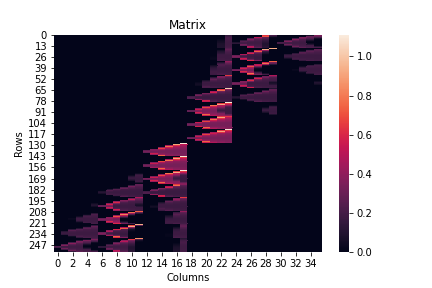
\includegraphics[width=0.5\textwidth]{A_1.png}
	\caption{Исходная матрица. Задача 2.1}
\end{figure}

Из графика матрицы видно, что она представляет собой комбинацию 4 блоков, 2 из которых являются матрицами, состоящими только из нулей. Возьмем один из ненулевых блоков. \\

\begin{figure}[h]
	\centering
	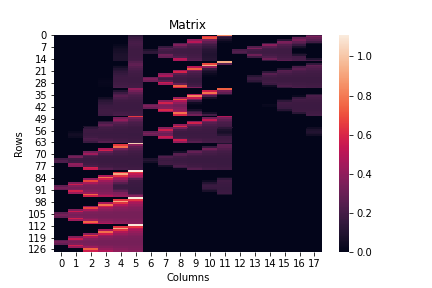
\includegraphics[width=0.5\textwidth]{A_block_1.png}
	\caption{Ненулевой блок исходной матрицы. Задача 2.1}
\end{figure}

В полученном блоке возьмем неособенный блок максимальной размерности. \\
\newpage
\begin{figure}[h]
	\centering
	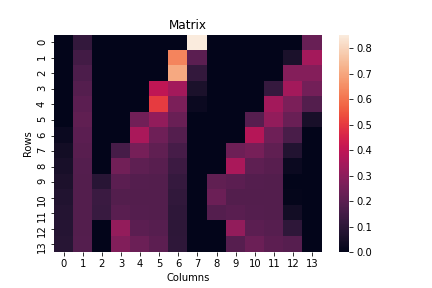
\includegraphics[width=0.5\textwidth]{A_subblock_1.png}
	\caption{Максимальный неособенный блок. Задача 2.1}
\end{figure}

Сгенерируем вектор $x$ с координатами из промежутка $ [1, 7]$. Получим вектор правой части $\textbf{b}=A_{block} x$. Сгенерируем вектор радиусов из интервала $[0.1, 1]$ и получим интервальную правую часть $\textbf{b}$. \\

Решим задачу с заданной точностью $\varepsilon=10^{-9}$ и максимальным количеством итераций 150. Полученный интервальный вектор-решение сравним с истинным решением. Кроме того сравним вектор правой части для полученного решения, истинный вектор правой части и интервальный истинный вектор правой части. Результаты представлены на графиках. \\
Количество итераций работы метода - 151. \\

\begin{figure}[h]
	\centering
	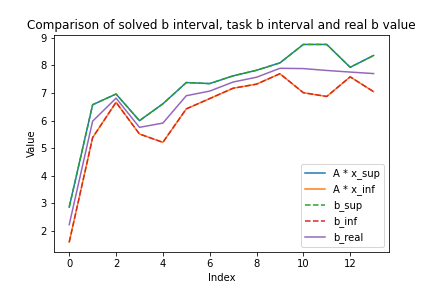
\includegraphics[width=0.5\textwidth]{solutions_1.png}
	\caption{Сравнение правых частей. Задача 2.1}
\end{figure}
\newpage
\begin{figure}[h]
	\centering
	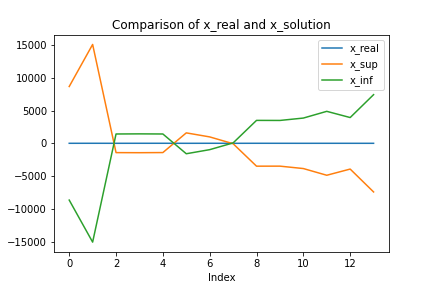
\includegraphics[width=0.5\textwidth]{xs_1.png}
	\caption{Сравнение векторов-решений. Задача 2.1}
\end{figure}

\begin{figure}[h]
	\centering
	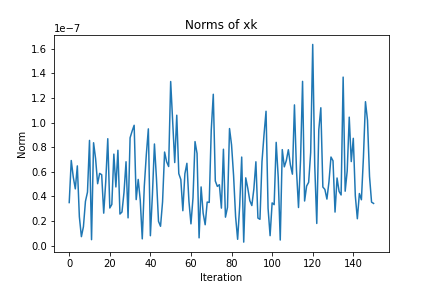
\includegraphics[width=0.5\textwidth]{norms_1.png}
	\caption{Сходимость метода. Задача 2.1}
\end{figure}

\subsection{Задача 2.2}
Повторим шаги из предыдущего пункта. Получим следующие результаты: \\
Количество итераций работы метода - 2.
\newpage
\begin{figure}[h]
	\centering
	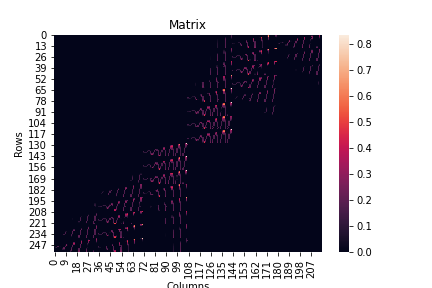
\includegraphics[width=0.5\textwidth]{A_6.png}
	\caption{Исходная матрица. Задача 2.2}
\end{figure}

\begin{figure}[h]
	\centering
	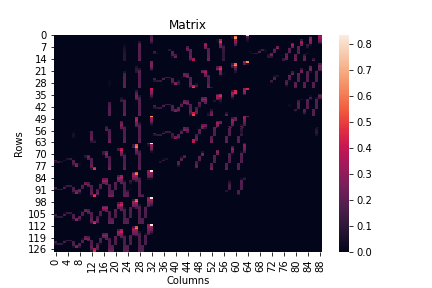
\includegraphics[width=0.5\textwidth]{A_block_6.png}
	\caption{Ненулевой блок исходной матрицы. Задача 2.2}
\end{figure}
\newpage
\begin{figure}[h]
	\centering
	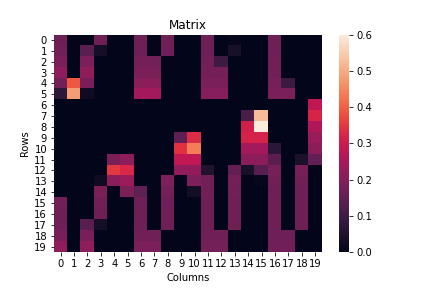
\includegraphics[width=0.5\textwidth]{A_subblock_6.png}
	\caption{Максимальный неособенный блок. Задача 2.2}
\end{figure}

\begin{figure}[h]
	\centering
	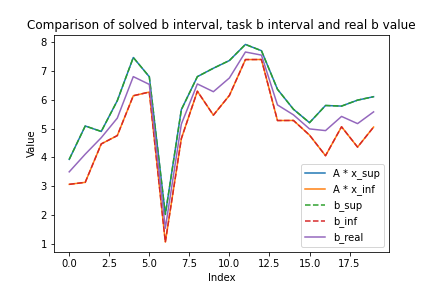
\includegraphics[width=0.5\textwidth]{solutions_6.png}
	\caption{Сравнение правых частей. Задача 2.2}
\end{figure}
\newpage
\begin{figure}[h]
	\centering
	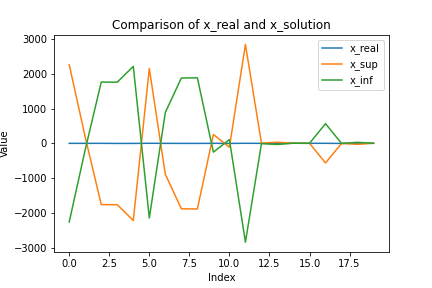
\includegraphics[width=0.5\textwidth]{xs_6.png}
	\caption{Сравнение векторов-решений. Задача 2.2}
\end{figure}

\begin{figure}[h]
	\centering
	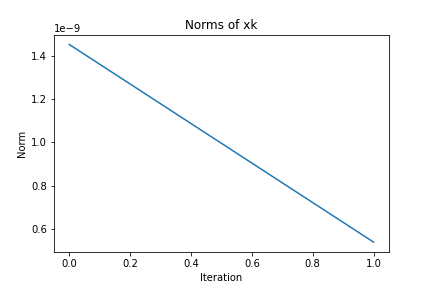
\includegraphics[width=0.5\textwidth]{norms_6.png}
	\caption{Сходимость метода. Задача 2.2}
\end{figure}


\section{Анализ}
\subsection{Задача 1}
Из результатов видно, что метод находит правильное решение: правые части совпали. Кроме того, поиск начального приближения дал практически сразу верное решение.

\subsection{Задача 2}
Полученные векторы-решения содержат в себе неправильные интервалы, что видно на графике со сравнением векторов-решений. Кроме того, границы полученных интервалов оказались во много раз больше значений координат истинного вектора решений. Тем не менее, как видно из графика со сравнением правых частей, полученные решения являются абсолютно верными. \\
Что касается сходимости, как и для задачи 1, поиск начального приближения дает практически сразу верное решение. Из графика со сходимостью для задачи 2.1 видно, что метод пытается удовлетворить условию окончания, но не справляется. Получаемые $x^{(k)}$ слабо отличаются друг от друга, но недостаточно, чтобы алгоритм завершился. Поэтому видны скачки, а окончание работы происходит лишь из-за достижения максимального количества итераций. Для задачи 2.2 условие окончания достигается на первой же итерации.

\section{Приложение}
Код программы на Python лежит в данном репозитории: \\
\url{https://github.com/PinkOink/Interval_Analysis/tree/main/lab5}{}


\end{document}